\section{Результати застосування розробленої системи}
\subsection{Стислі відомості щодо розгортання системи}

Вимоги до серверної машини наведено у таблиці~\ref{tab:sw_requirements}. 

\begin{table}[h]
	\caption{Мінімальні вимоги до серверного обладнання}
	\label{tab:sw_requirements}
	\begin{tabular}{l|l}
		Процесор & 1000 МГц \\ \hline
		ОЗП & 512 МБ \\ \hline
		Об'єм пам'яті диску & 64 ГБ 
	\end{tabular}
\end{table}

Програмне забезпечення серверу може бути встановлено на операційні системи родини \textit{Linux}, \textit{Windows} або \textit{macOS}.
Рекомендовано використовувати \acrshort{ssd} у якості накопичувача.

Для розгортання системи необхідно встановити наступні програми:
\begin{itemize}
	\item Apache Server v2.4.29+;
	\item SQLite v3.22.0+;
	\item PHP v7.2.2+;
\end{itemize}
та встановити драйвер взаємодії PHP з SQLite.

\subsection{Опис роботи з сайтом}
Робота з сайтом починається з процесу реєстрації користувача~(рисунок~\ref{fig:site_register}).
Незареєстрований користувач може переглядати товари та додавати їх до кошику, але не може оформити замовлення. 
\begin{figure}[H]
    \centering
    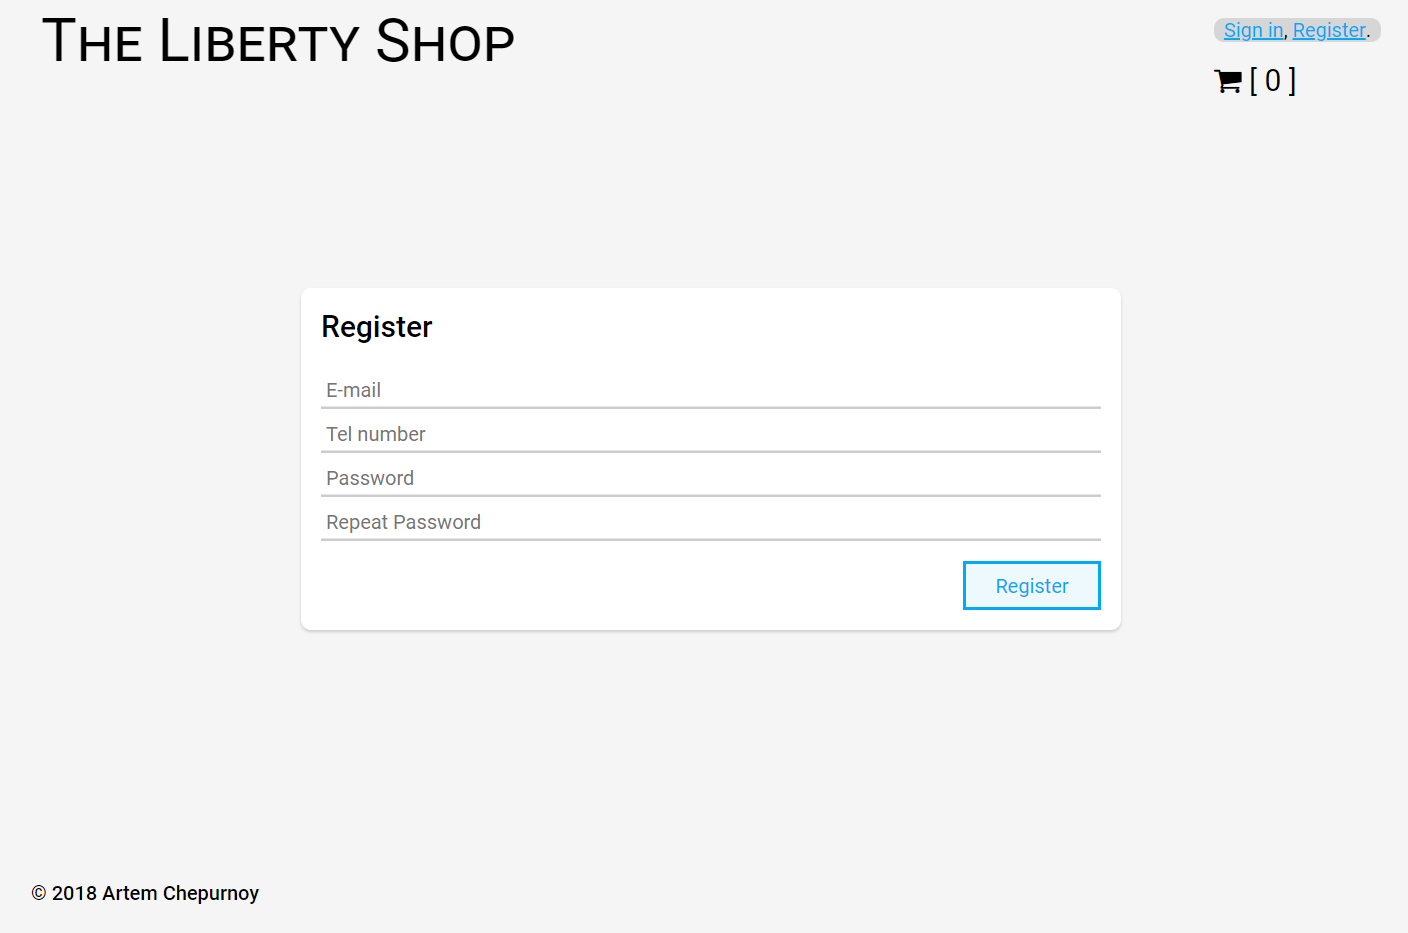
\includegraphics[width=0.8\textwidth]{screen_register}
    \caption{Сторінка реєстрації у системі}
    \label{fig:site_register}
\end{figure}

Після реєстрації користувач має увійти до системи~(рисунок~\ref{fig:site_login}).
\begin{figure}[H]
    \centering
    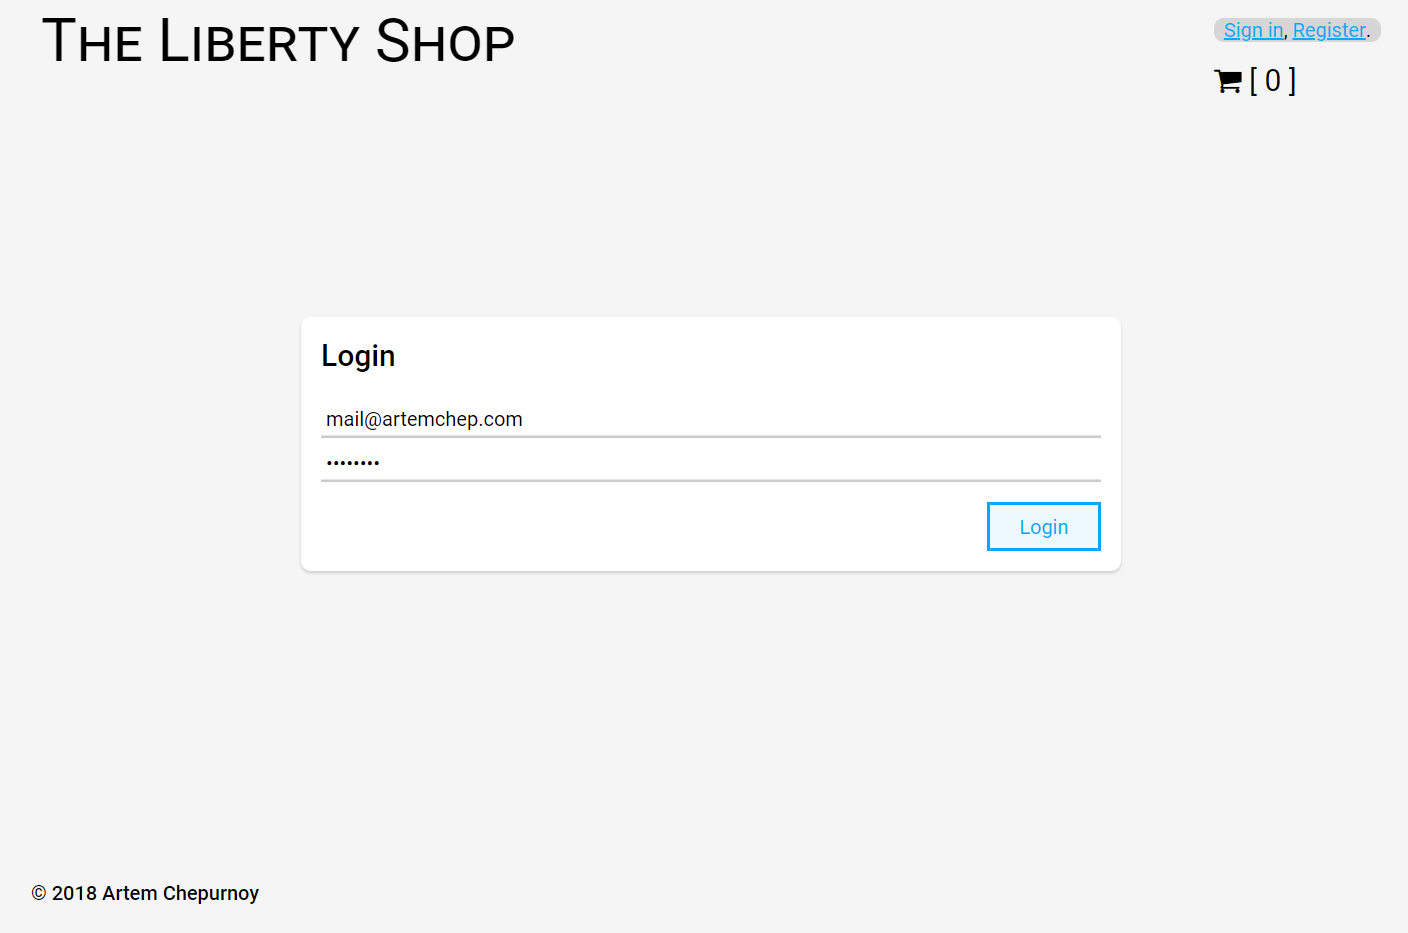
\includegraphics[width=0.8\textwidth]{screen_login}
    \caption{Сторінка входу до системи}
    \label{fig:site_login}
\end{figure}

Користувач може переглядати доступні товари на головній сторінці сайту.
Доступна можливість пошуку товару за ім'ям та категоріям.
\begin{figure}[H]
    \centering
    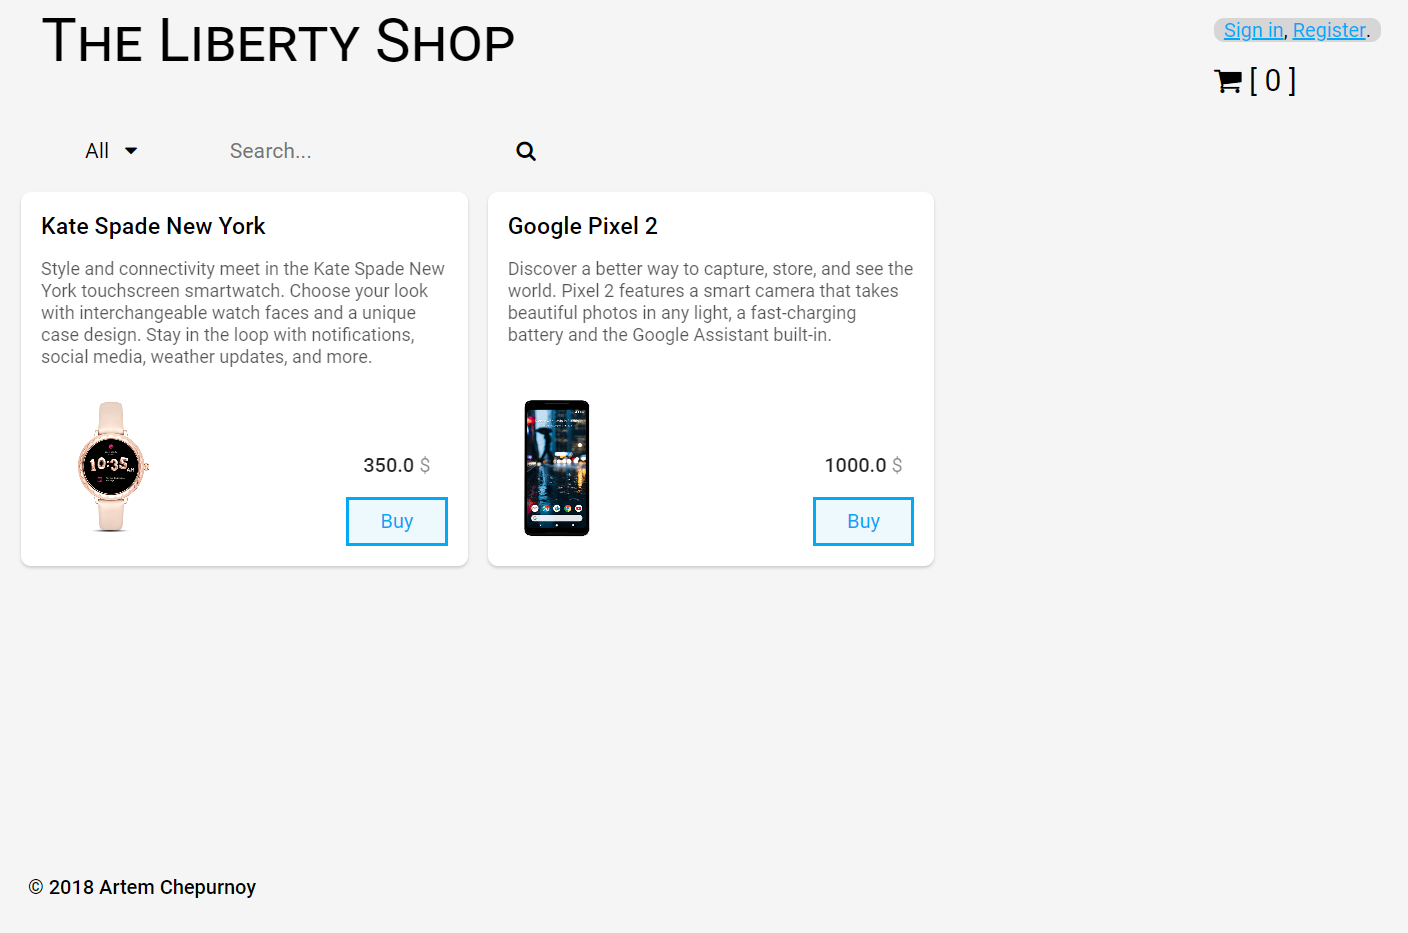
\includegraphics[width=0.8\textwidth]{screen_product__list}
    \caption{Головна сторінка ресурсу}
    \label{fig:site_product_list}
\end{figure}

Адміністратор та менеджери сайту мають на головній сторінці додаткові елементи~(рисунок~\ref{fig:site_product_list_admin}): 
\begin{itemize}
\item Кнопка редагування продуктів;
\item \textit{<<Add product>>} --- показати діалог додавання нового продукту;
\item \textit{<<Add category>>} --- показати діалог додавання нової категорії продуктів;
\item \textit{<<Edit category>>} --- показати діалог редагування та видалення категорії продуктів.
\end{itemize}
\begin{figure}[H]
    \centering
    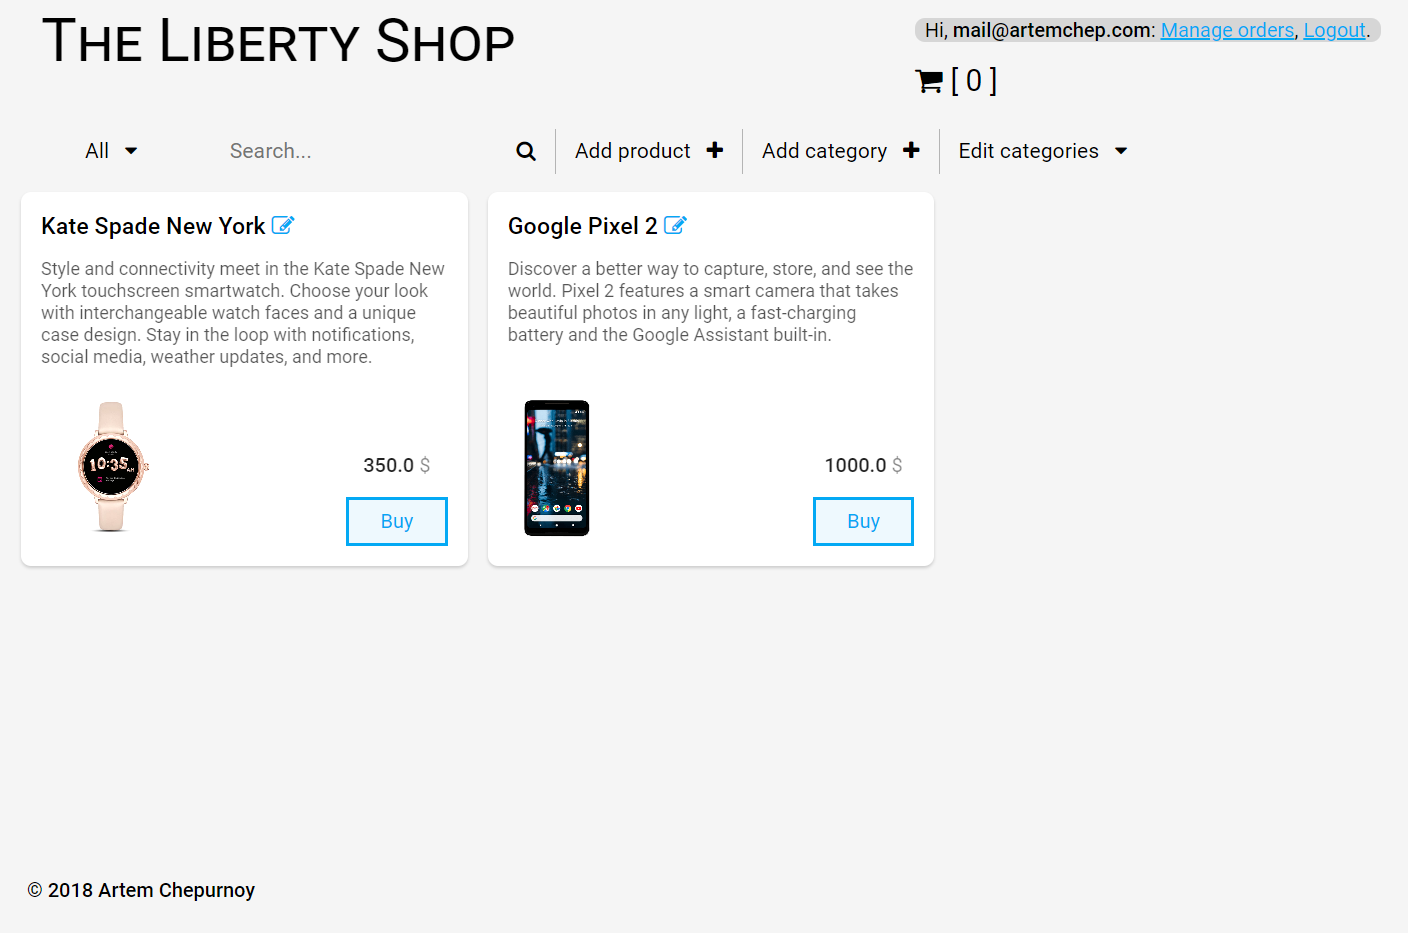
\includegraphics[width=0.8\textwidth]{screen_product__list__admin}
    \caption{Головна сторінка ресурсу (адміністратор)}
    \label{fig:site_product_list_admin}
\end{figure}

Діалог для створення нового продукту представлено на рисунку~\ref{fig:site_product_add}).

Продукт має такі властивості як категорія продуктів, назва, короткий опис, графічне зображення, ціна та розмірність.   
\begin{figure}[H]
    \centering
    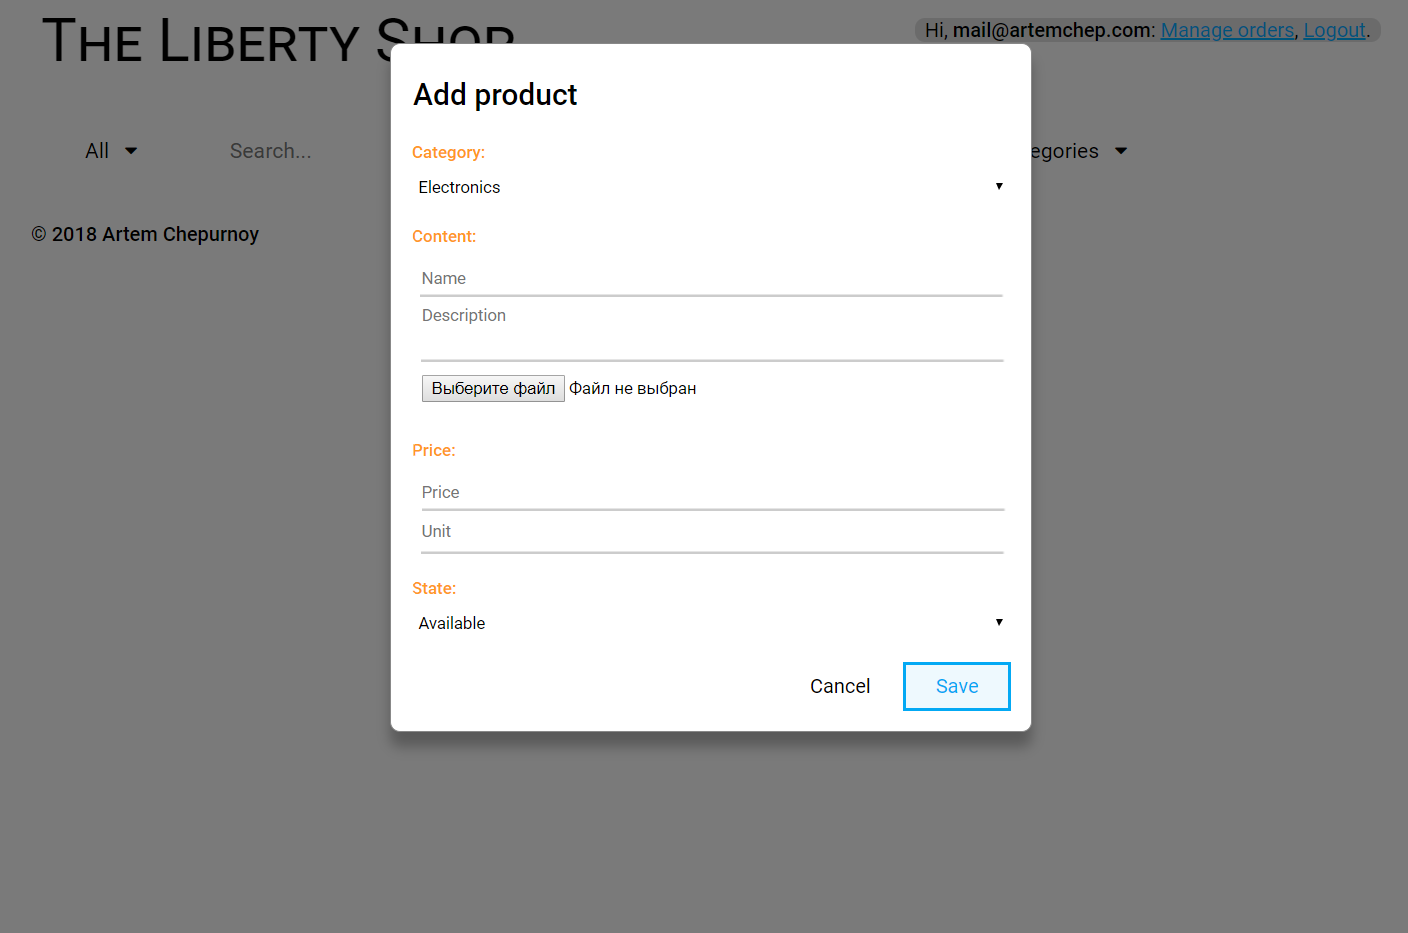
\includegraphics[width=0.8\textwidth]{screen_product_add}
    \caption{Діалог створення нового продукту}
    \label{fig:site_product_add}
\end{figure}

Адміністратор та менеджер ресурсу мають можливість переглянути список поточних або минулих замовлень~(рисунок~\ref{fig:site_order_list}), перемістити замовлення до архіву.
Є можливість фільтрування замовлень по даті створення, даті архівування, назві, категорії, кількості продуктів та ціні.   
\begin{figure}[H]
    \centering
    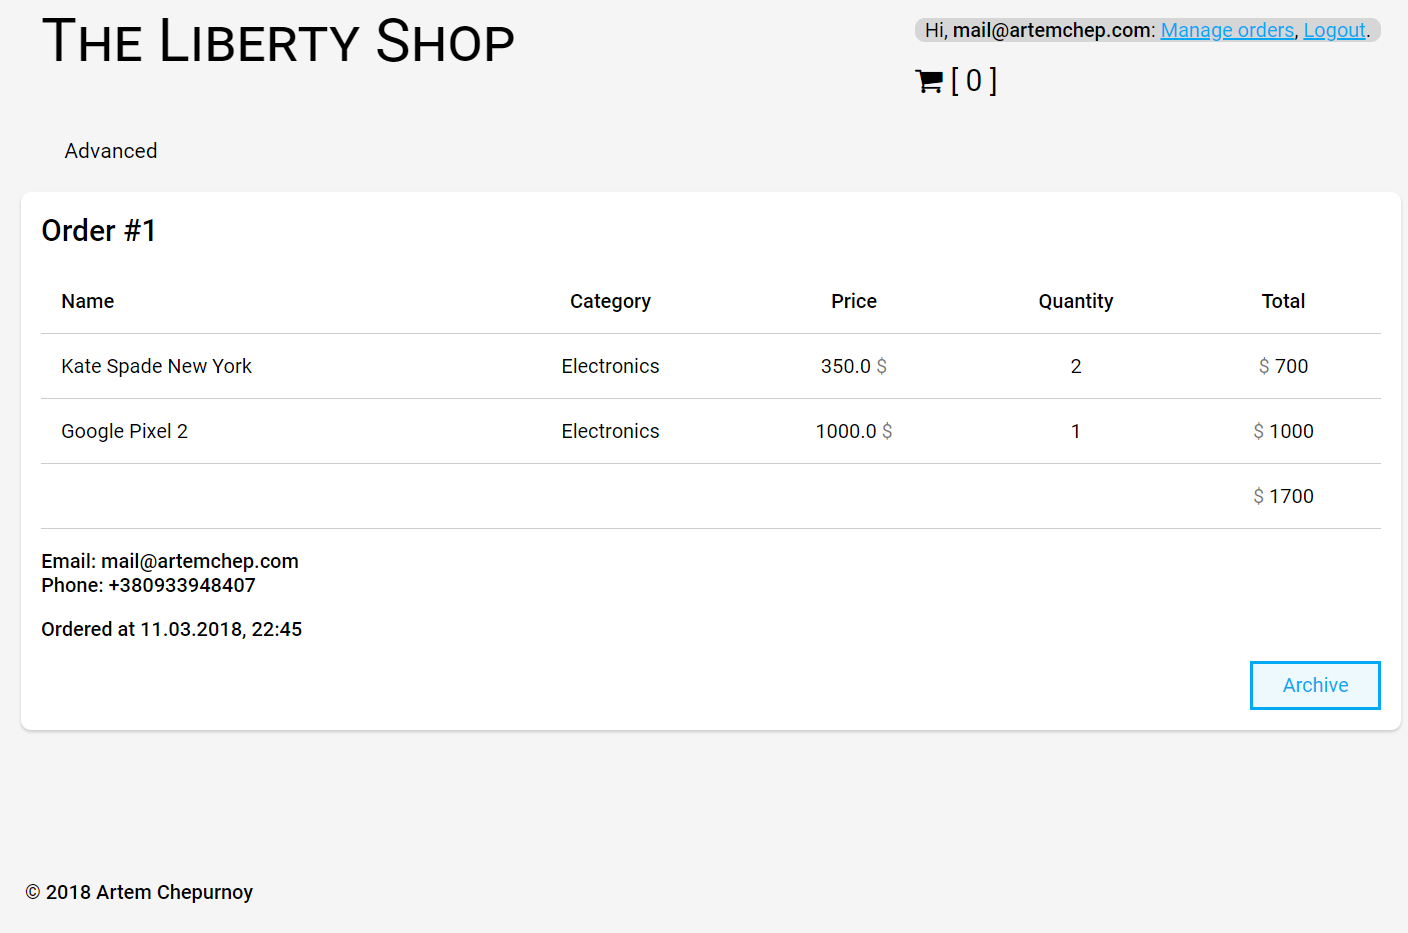
\includegraphics[width=0.8\textwidth]{screen_order__list}
    \caption{Сторінка керування замовленнями}
    \label{fig:site_order_list}
\end{figure}

\subsection{Результати тестування та рекомендації щодо удосконалення розробленої системи}
При тестуванні основною проблемою виявилася підтримка сайтом різних пристроїв та браузерів. 
При більш детальному вивченні стандартів HTML та CSS ця проблема була вирішена.

Одним із напрямків розвитку розробленої системи є співробітництво з іншими постачальниками, створення платформи для постачальників. 
